\chapter{Stochastic optimal power flow (SOPFLOW)}\label{chap:sopflow}
SOPFLOW solves a stochastic security-constrained multi-period optimal power flow problem. The problem is set up as a two-stage optimization problem where the first-stage (base-case) represents the normal operation of the grid (or the most likely forecast) and the second-stage comprises $N_s$ scenarios of forecast deviation. Each scenario can have multiple contingencies and each contingency can be multi-period.

\section{Formulation}
An illustration of \sopflow is shown in Fig. \ref{fig:sctopflow} for a case with two scenarios $s_0$ and $s_1$ with three contingencies each, and each scenario/contingency with two time-periods. We assume that any contingency is incident at the first time-step, i.e., at $t_0$.


\definecolor{lavander}{cmyk}{0,0.48,0,0}
\definecolor{violet}{cmyk}{0.79,0.88,0,0}
\definecolor{burntorange}{cmyk}{0,0.52,1,0}

\def\lav{lavander!90}
\def\oran{orange!30}

\tikzstyle{contingency}=[draw,circle,violet,bottom color=\lav,
                  top color= white, text=violet,minimum width=50pt]
\tikzstyle{base}=[draw,circle,burntorange, left color=\oran,
                       text=violet,minimum width=50pt]

\tikzstyle{time}=[draw,circle,blue,text=violet,minimum width=2pt]
\tikzstyle{tbase}=[draw,circle,burntorange, left color=\oran,
                            text=violet,minimum width=2pt]
                       
\tikzstyle{cedge}=[color=red]

\begin{figure}[h!]
\centering
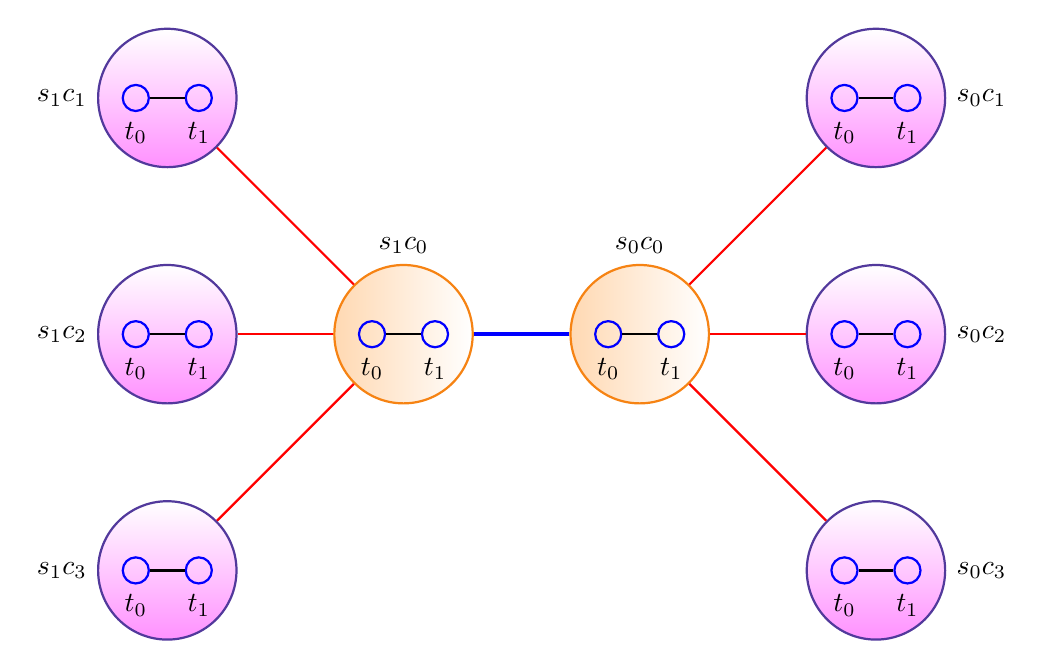
\begin{tikzpicture}[auto, thick]
  % Place base case
  \node[base,label=above:$s_0c_0$] (s0c0) at (1,0) {};
  \node[time,label=below:$t_0$] (s0c0t0) at (0.6,0) {};
  \node[time,label=below:$t_1$] (s0c0t1) at (1.4,0) {};
  
  \node[contingency,label=right:$s_0c_1$] (s0c1) at (4,3) {};
  \node[time,label=below:$t_0$] (s0c1t0) at (3.6,3) {};
  \node[time,label=below:$t_1$] (s0c1t1) at (4.4,3) {};

  \node[contingency,label=right:$s_0c_2$] (s0c2) at (4,0) {};
  \node[time,label=below:$t_0$] (s0c2t0) at (3.6,0) {};
  \node[time,label=below:$t_1$] (s0c2t1) at (4.4,0) {};

  
  \node[contingency,label=right:$s_0c_3$] (s0c3) at (4,-3) {};
  \node[time,label=below:$t_0$] (s0c3t0) at (3.6,-3) {};
  \node[time,label=below:$t_1$] (s0c3t1) at (4.4,-3) {};
  
  \path (s0c0t0) edge (s0c0t1);
  \path (s0c1t0) edge (s0c1t1);
  \path (s0c2t0) edge (s0c2t1);
  \path (s0c3t0) edge (s0c3t1);
  
  \path[cedge] (s0c0) edge (s0c1);
  \path[cedge] (s0c0) edge (s0c2);
  \path[cedge] (s0c0) edge (s0c3);

  % Second scenario
  \node[base,label=above:$s_1c_0$] (s1c0) at (-2,0) {};
  \node[time,label=below:$t_0$] (s1c0t0) at (-2.4,0) {};
  \node[time,label=below:$t_1$] (s1c0t1) at (-1.6,0) {};
  
  \node[contingency,label=left:$s_1c_1$] (s1c1) at (-5,3) {};
  \node[time,label=below:$t_0$] (s1c1t0) at (-5.4,3) {};
  \node[time,label=below:$t_1$] (s1c1t1) at (-4.6,3) {};

  \node[contingency,label=left:$s_1c_2$] (s1c2) at (-5,0) {};
  \node[time,label=below:$t_0$] (s1c2t0) at (-5.4,0) {};
  \node[time,label=below:$t_1$] (s1c2t1) at (-4.6,0) {};

  
  \node[contingency,label=left:$s_1c_3$] (s1c3) at (-5,-3) {};
  \node[time,label=below:$t_0$] (s1c3t0) at (-5.4,-3) {};
  \node[time,label=below:$t_1$] (s1c3t1) at (-4.6,-3) {};
  
  \path (s1c0t0) edge (s1c0t1);
  \path (s1c1t0) edge (s1c1t1);
  \path (s1c2t0) edge (s1c2t1);
  \path (s1c3t0) edge (s1c3t1);
  
  \path[cedge] (s1c0) edge (s1c1);
  \path[cedge] (s1c0) edge (s1c2);
  \path[cedge] (s1c0) edge (s1c3);

  \path (s0c0) edge [ultra thick,color=blue] (s1c0);

\end{tikzpicture}

\caption{Stochastic multi-period contingency constrained structure with two scenarios $s_0$ and $s_1$. Each scenario has three contingencies $c_1$,$c_2$,and $c_3$. $s_0c_0$ and $s_1c_0$ denote the base-cases for the two scenarios. Each scenario and contingency has two time-periods $t_0$, and $t_2$, $t_2$. The {\textcolor{red}{red}} line denotes the coupling between the contingencies and their respective base-case scenarios.The {\textcolor{blue}{blue}} line denotes the coupling between the scenarios}
\label{fig:sctopflow}
\end{figure}


The full formulation for the stochastic security-constrained multi-period optimal power flow is given in (\ref{eq:sctopflow_start}) -- (\ref{eq:sctopflow_end}). In this formulation, the objective is to reduce the expected cost, where $f(x_{s,c,t})$ is the cost for scenario $s$ with contingency $c$ at time $t$. $\pi_s$ is the probability of scenario $s$.

\begin{align}
\centering
\text{min}&~\sum_{s=0}^{N_s-1}\pi_s\sum_{c=0}^{N_c-1}\sum_{t=0}^{N_t-1}f(x_{s,c,t})&  \label{eq:sctopflow_start}\\
&\text{s.t.}& \nonumber \\
&~g(x_{s,c,t}) = 0,                                        &s \in \left[1,N_s-1\right],c \in \left[0,N_c-1\right], t \in \left[0,N_t-1\right]& \\
&~h(x_{s,c,t}) \le 0,                                      &s \in \left[1,N_s-1\right],c \in \left[0,N_c-1\right], t \in \left[0,N_t-1\right]& \\
x^- & \le x_{s,c,t} \le x^+,                               &s \in \left[1,N_s-1\right],c \in \left[0,N_c-1\right], t\in \left[0,N_t-1\right]& \\
-\Delta x_t & \le x_{s,c,t} - x_{s,c,t-\Delta{t}} \le \Delta x_t,&s \in \left[1,N_s-1\right],c \in \left[0,N_c-1\right], t \in \left[1,N_t-1\right]& \label{eq:sctopflow_time_coupling}\\
-\Delta x_c & \le x_{s,c,0} - x_{s,0,0} \le \Delta x_c,&s \in \left[1,N_s-1\right],c \in \left[1,N_c-1\right]&
\label{eq:sctopflow_contingency_coupling} \\
-\Delta x_s & \le x_{s,0,0} - x_{0,0,0} \le \Delta x_s,&s \in \left[1,N_s-1\right]&
\label{eq:sctopflow_end}
\end{align}

The modeling details used for an optimial power flow problem are also used for a {\sopflow} problem, i.e., each of the circles shown in Fig. \ref{fig:sctopflow} has the modeling details of an optimal power flow problem (\opflow). Incorporating the probabilities $\pi_s$ for each scenario is not implemented yet which leads to each scenario having an equal probability. 

Depending on the options selected, SOPFLOW can be used to solve 
\begin{itemize}
    \item Single-period stochastic optimal power flow : No contingencies or time-periods
    \item Single-period contingency-constrained stochastic optimal power flow : No time-periods
    \item Multi-period security-constrained stochastic optimal power flow : Full formulation
\end{itemize}

Currently, \sopflow uses wind power generation as the stochastic variables and each scenario is a realization of the power output from wind generators. A zero fuel cost is used for wind power generation to ensure wind generation would be the dispatched to the given target level (upper limit). 

For contingencies, \sopflow supports generation and/or transmission outages. A contingency can have multiple outages, but, it should not cause any islanding. The coupling between the no-contingency and the contingency case for each scenario is also the difference in real power output ($p_{jsct}^{\text{g}} - p_{js0t}^{\text{g}},~ \jinJgen$) that must be within the 30 minute generator ramp rate. Refer to \ref{chap:scopflow} for details on the contingency modeling.

For multi time-period, we use ramping constraints on the generator real power output between successive time steps.

\sopflow can be run in two modes: preventive and corrective. In the preventive mode, generator real power output is fixed to the base-case values for generators at PV bus(es). In this mode, the generators at the reference bus provide/absorb any deficit/surplus power. The corrective mode allows deviation of the PV and PQ generator real power from the base-case dispatch constrained by its 30-min. ramp rate capability. Note that the preventive/corrective mode is only applied at the first step $t_0$. In the successive time-steps, the generator dispatch is dictated by the previous step dispatch and the ramp limits.

\section{Solvers}
\sopflow can be solved with \ipopt. If one wants to solve each scenario independently, i.e., without any coupling constraints then use the \emph{EMPAR} solver. \emph{EMPAR} distributes the contingencies to different processes when executed in parallel.

\section{Input and Output}
The following files are needed for executing SOPFLOW.
\begin{itemize}
    \item \textbf{Network file:} The network file describing the network details. Only \matpower format files are currently supported.
    \item \textbf{Scenario file:} \sopflow only supports reading wind generation scenarios in a CSV format. An example of this format for the 9-bus case is \href{https://gitlab.pnnl.gov/exasgd/frameworks/exago/-/tree/master/datafiles/case9/scenarios_9bus.csv}{here}.
    \item \textbf{Contingency file:} Contingencies can be specified via PTI format file as described in chapter \ref{chap:scopflow}. The option \lstinline{-sopflow_enable_multicontingency} should be set for multi-contingency problems.
    \item \textbf{Load data:} One file for load real power and one for reactive power. The files need to be in CSV format. An example of the format for the 9-bus case is \href{https://gitlab.pnnl.gov/exasgd/frameworks/exago/-/tree/master/datafiles/case9}{here}.
\end{itemize}

The \sopflow output is saved to a directory named \texttt{sopflowout}. This
directory contains $N_s$ subdirectories to save the solution for each scenario.
Each of these subdirectories contain $N_c$ subdirectories, one for each
contingency. Each contingency subdirectory has $N_t$ MATPOWER format files to
store the output for each time-period for the given contingency and scenario.
The subdirectories have the directory name format \texttt{scen_x} where x is
the scenario number,  \texttt{cont_y} where y is the contingency number, and
the output files have the file name format \texttt{t_z} where z is the time-step number.

\section{Usage}
\begin{lstlisting}
    ./sopflow -netfile <netfilename>  -scenfile <scenfilename> \
    [-sopflow_enable_multicontingency 1] <sopflowoptions>
\end{lstlisting}

\section{Options}

\begin{table}[!htbp]
  \caption{SOPFLOW options}
  \small
  \begin{tabular}{|p{0.3\textwidth}|p{0.3\textwidth}|p{0.3\textwidth}|}
    \hline
    \textbf{Option} & \textbf{Meaning} & \textbf{Values (Default value)} \\ \hline
    -netfile & Network file name & string $<$ 4096 characters (\href{https://gitlab.pnnl.gov/exasgd/frameworks/exago/-/blob/master/datafiles/case9/case9mod_gen3_wind.m}{case9mod\_gen3\_wind.m}) \\ \hline
    -scenfile & Scenario file name & string $<$ 4096 characters (\href{https://gitlab.pnnl.gov/exasgd/frameworks/exago/-/blob/master/datafiles/case9/scenarios_9bus.csv}{case9/scenarios\_9bus.csv}) \\ \hline
    -sopflow\_mode & Operation mode: Preventive or corrective & 0 or 1 (0) \\ \hline
    -sopflow\_solver & Set solver for sopflow & IPOPT or  EMPAR \\ \hline
    -sopflow\_enable\_multicontingency & Multi-contingency SOPFLOW & 0 or 1 (0) \\ \hline
    -ctgcfile & Contingency file name & string (\href{https://gitlab.pnnl.gov/exasgd/frameworks/exago/-/blob/master/datafiles/case9/case9.cont}{case9.cont}) \\ \hline
    -sopflow\_Ns & Number of scenarios & int (Default 0. Use -1 to select all scenarios from the scenario file) \\ \hline
  \end{tabular}
  \label{tab:sopflow_options}
\end{table}

%See table \ref{tab:sopflow_options}. With multi-contingency SOPFLOW, all \scopflow options given in Table \ref{tab:scopflow_options} can be used to tune the contingencies. All \opflow options in Table \ref{tab:opflow_options}, along with \tcopflow options in Table \ref{tab:tcopflow_options} can also be used. Multi-contingency SOPFLOW also allows the options listed after -sopflow\_enable\_multicontingency in Table \ref{tab:sopflow_options} to be used.

Depending on the \emph{mode}, SOPFLOW can either be \emph{preventive} (mode = 0) or \emph{corrective} (mode = 1). In the preventive mode, the PV and PQ generator real power is fixed to its corresponding base-case values. The generators at the reference bus pick up any make-up power required for the contingency. The corrective mode allows deviation of the PV and PQ generator real power from the base-case dispatch constrained by its 30-min. ramp rate capability.

\section{Examples}
Some \sopflow example runs are provided with some sample output. Options are the default options given in Tables \ref{tab:opflow_options}, \ref{tab:tcopflow_options}, \ref{tab:scopflow_options} and \ref{tab:sopflow_options} unless otherwise specified. Sample output is generated by running examples in the installation directory.

Example using the \ipopt solver:

\begin{lstlisting}
$ ./bin/sopflow -print_output -sopflow_solver IPOPT
[ExaGO INFO]: -- Checking ... -options_file not passed    exists: no
SOPFLOW: Application created
Rank[0]: color = 0, ns = 2, sstart= 0, send=2
SOPFLOW running with 2 scenarios (base case + 1 scenarios)
Rank 0 scenario range [0 -- 2]
SOPFLOW: Using IPOPT solver
SOPFLOW: Setup completed

********************************************************************
This program contains Ipopt, a library for large-scale nonlinear 
optimization. Ipopt is released as open source code under the 
Eclipse Public License (EPL).
********************************************************************

This is Ipopt version 3.12.10, running with linear solver ma27.

Number of nonzeros in equality constraint Jacobian...:      222
Number of nonzeros in inequality constraint Jacobian.:      168
Number of nonzeros in Lagrangian Hessian.............:      180

Total number of variables............................:       46
                     variables with only lower bounds:        0
                variables with lower and upper bounds:       30
                     variables with only upper bounds:        0
Total number of equality constraints.................:       37
Total number of inequality constraints...............:       50
        inequality constraints with only lower bounds:       12
   inequality constraints with lower and upper bounds:       38
        inequality constraints with only upper bounds:        0

iter  objective  inf_pr  inf_du lg(mu) ||d|| lg(rg) alpha_du alpha_pr  ls
0  1.4884250e+04 1.80e+00 5.02e+01  -1.0 0.00e+00 - 0.00e+00 0.00e+00   0
1  1.0889088e+04 1.45e+00 7.87e+01  -1.0 1.92e+00 - 1.69e-01 1.93e-01f  1
2  1.0548318e+04 1.33e+00 7.28e+01  -1.0 6.01e-01 - 2.76e-02 8.30e-02f  1
...
29  5.9075224e+03 1.24e-14 2.96e-12 -7.0 4.91e-10 - 1.00e+00 1.00e+00h  1

Number of Iterations....: 29

                                   (scaled)                 (unscaled)
Objective...........:   1.3245566021454471e+02    5.9075224455686939e+03
Dual infeasibility..:   2.9592247352450450e-12    1.3198142319192901e-10
Constraint violation:   1.2434497875801753e-14    1.2434497875801753e-14
Complementarity.....:   9.0910764708133484e-08    4.0546201059827535e-06
Overall NLP error...:   9.0910764708133484e-08    4.0546201059827535e-06


Number of objective function evaluations             = 33
Number of objective gradient evaluations             = 30
Number of equality constraint evaluations            = 33
Number of inequality constraint evaluations          = 33
Number of equality constraint Jacobian evaluations   = 30
Number of inequality constraint Jacobian evaluations = 30
Number of Lagrangian Hessian evaluations             = 29
Total CPU secs in IPOPT (w/o function evaluations)   =      0.006
Total CPU secs in NLP function evaluations           =      0.003

EXIT: Optimal Solution Found.
=============================================================
        Stochastic Optimal Power Flow
=============================================================
OPFLOW Formulation                  POWER_BALANCE_POLAR
Solver                              IPOPT
Initialization                      MIDPOINT
Number of scenarios                 1
Load loss allowed                   NO
Power imbalance allowed             NO
Ignore line flow constraints        NO

Number of variables                 48
Number of equality constraints      0
Number of inequality constraints    0
Number of coupling constraints      0

Convergence status                  CONVERGED
Objective value                     5907.52

----------------------------------------------------------------------
Bus        Pd      Qd      Vm      Va      mult_Pmis      mult_Qmis
----------------------------------------------------------------------
1         0.00    0.00   1.040   0.000      2218.76        -0.00
2         0.00    0.00   1.025   4.156      2170.20         0.00
3         0.00    0.00   1.025   1.685      2180.00         0.00
4         0.00    0.00   1.038  -2.389      2219.06        -0.56
5        75.00   30.00   1.026  -3.714      2231.93         2.96
6        90.00   30.00   1.023  -4.683      2252.92         4.40
7         0.00    0.00   1.033   0.291      2170.95         4.07
8       100.00   35.00   1.022  -2.352      2196.02         8.01
9         0.00    0.00   1.036  -0.689      2180.43         2.83

--------------------------------------------------------------------------
From       To       Status     Sft      Stf     Slim     mult_Sf  mult_St
--------------------------------------------------------------------------
1          4          1       78.31    78.15   380.00    -0.00    -0.00
2          7          1      114.58   115.48   250.00    -0.00    -0.00
3          9          1       76.90    77.69   300.00    -0.00    -0.00
4          5          1       30.36    36.13   250.00    -0.00    -0.00
4          6          1       47.82    49.77   250.00    -0.00    -0.00
5          7          1       45.94    49.28   250.00    -0.00    -0.00
6          9          1       45.11    47.63   150.00    -0.00    -0.00
7          8          1       68.77    69.83   250.00    -0.00    -0.00
8          9          1       37.83    31.76   150.00    -0.00    -0.00

-------------------------------------------------------------------------
Gen  Status    Fuel     Pg       Qg       Pmin     Pmax     Qmin     Qmax
-------------------------------------------------------------------------
1     1        COAL    78.13     5.42    10.00   350.00  -300.00   300.00
2     1        COAL   114.18    -9.55    10.00   300.00  -300.00   300.00
3     1        WIND    75.00   -17.00     0.00    75.00  -300.00   300.00
[ExaGO INFO]: Finalizing sopflow application.
\end{lstlisting}

Example using the \emph{EMPAR} solver with multicontingency enabled:

\begin{lstlisting}
$ ./bin/sopflow -sopflow_solver EMPAR -sopflow_enable_multicontingency 1
[ExaGO INFO]: -- Checking ... -options_file not passed       exists: no
SOPFLOW: Application created
Rank[0]: color = 0, ns = 2, sstart= 0, send=2
SOPFLOW running with 2 scenarios (base case + 1 scenarios)
Rank 0 scenario range [0 -- 2]
SOPFLOW: Using EMPAR solver
SCOPFLOW: Application created
SCOPFLOW running with 2 contingencies (base case + 1 contingencies)
Rank 0 has 2 contingencies, range [0 -- 2]
SCOPFLOW: Using IPOPT solver
SCOPFLOW: Setup completed
SCOPFLOW: Application created
SCOPFLOW running with 2 contingencies (base case + 1 contingencies)
Rank 0 has 2 contingencies, range [0 -- 2]
SCOPFLOW: Using IPOPT solver
SCOPFLOW: Setup completed
SOPFLOW: Setup completed

**********************************************************************
This program contains Ipopt, a library for large-scale nonlinear 
optimization. Ipopt is released as open source code under the 
Eclipse Public License (EPL).
**********************************************************************

This is Ipopt version 3.12.10, running with linear solver ma27.

Number of nonzeros in equality constraint Jacobian...:      226
Number of nonzeros in inequality constraint Jacobian.:      168
Number of nonzeros in Lagrangian Hessian.............:      215

Total number of variables............................:       51
                     variables with only lower bounds:        0
                variables with lower and upper bounds:       35
                     variables with only upper bounds:        0
Total number of equality constraints.................:       42
Total number of inequality constraints...............:       58
        inequality constraints with only lower bounds:       21
   inequality constraints with lower and upper bounds:       37
        inequality constraints with only upper bounds:        0

iter  objective  inf_pr  inf_du lg(mu) ||d|| lg(rg) alpha_du alpha_pr  ls
0  7.4421250e+03 1.80e+00 1.04e+01  -1.0 0.00e+00 - 0.00e+00 0.00e+00   0
1  6.5388630e+03 1.51e+00 2.24e+01  -1.0 1.07e+00 - 5.38e-01 1.58e-01f  1
2  5.9394843e+03 1.28e+00 2.56e+02  -1.0 7.32e-01 - 3.31e-02 1.56e-01f  1
...
29  3.0556401e+03 1.07e-14 5.62e-10  -8.6 4.33e-09 - 1.00e+00 1.00e+00f 1

Number of Iterations....: 29

                                   (scaled)                 (unscaled)
Objective...........:   6.8512110964678271e+01    3.0556401490246512e+03
Dual infeasibility..:   5.6231688979129259e-10    2.5079333284691651e-08
Constraint violation:   1.0658141036401503e-14    1.0658141036401503e-14
Complementarity.....:   2.7880113972390153e-09    1.2434530831686009e-07
Overall NLP error...:   2.7880113972390153e-09    1.2434530831686009e-07


Number of objective function evaluations             = 48
Number of objective gradient evaluations             = 30
Number of equality constraint evaluations            = 48
Number of inequality constraint evaluations          = 48
Number of equality constraint Jacobian evaluations   = 30
Number of inequality constraint Jacobian evaluations = 30
Number of Lagrangian Hessian evaluations             = 29
Total CPU secs in IPOPT (w/o function evaluations)   =      0.010
Total CPU secs in NLP function evaluations           =      0.006

EXIT: Optimal Solution Found.
This is Ipopt version 3.12.10, running with linear solver ma27.

Number of nonzeros in equality constraint Jacobian...:      226
Number of nonzeros in inequality constraint Jacobian.:      168
Number of nonzeros in Lagrangian Hessian.............:      215
Total number of variables............................:       51
                     variables with only lower bounds:        0
                variables with lower and upper bounds:       35
                     variables with only upper bounds:        0
Total number of equality constraints.................:       42
Total number of inequality constraints...............:       58
        inequality constraints with only lower bounds:       21
   inequality constraints with lower and upper bounds:       37
        inequality constraints with only upper bounds:        0

iter objective  inf_pr  inf_du lg(mu) ||d|| lg(rg) alpha_du alpha_pr  ls
0  7.4421250e+03 1.80e+00 1.04e+01  -1.0 0.00e+00 - 0.00e+00 0.00e+00   0
1  6.2852600e+03 1.53e+00 2.73e+01  -1.0 1.34e+00 - 3.21e-01 1.50e-01f  1
...
28  2.8488309e+03 1.07e-14 3.60e-09 -8.6 1.94e-08 - 1.00e+00 1.00e+00h  1

Number of Iterations....: 28

                                (scaled)                 (unscaled)
Objective...........:   6.3875131478884526e+01    2.8488308639582501e+03
Dual infeasibility..:   3.5985088591418374e-09    1.6049349511772596e-07
Constraint violation:   1.0658141036401503e-14    1.0658141036401503e-14
Complementarity.....:   4.7446211848960068e-09    2.1161010484636192e-07
Overall NLP error...:   4.7446211848960068e-09    2.1161010484636192e-07


Number of objective function evaluations             = 43
Number of objective gradient evaluations             = 29
Number of equality constraint evaluations            = 43
Number of inequality constraint evaluations          = 43
Number of equality constraint Jacobian evaluations   = 29
Number of inequality constraint Jacobian evaluations = 29
Number of Lagrangian Hessian evaluations             = 28
Total CPU secs in IPOPT (w/o function evaluations)   =      0.016
Total CPU secs in NLP function evaluations           =      0.009

EXIT: Optimal Solution Found.
\end{lstlisting}

Example using the \ipopt solver with multicontingency and multiperiod enabled:

\begin{lstlisting}
./bin/sopflow -sopflow_solver IPOPT -sopflow_enable_multicontingency 1\
-scopflow_enable_multiperiod 1 -sopflow_Ns -1 -scopflow_Nc -1
[ExaGO INFO]: -- Checking ... -options_file not passed        exists: no
SOPFLOW: Application created
Rank[0]: color = 0, ns = 4, sstart= 0, send=4
SOPFLOW running with 4 scenarios (base case + 3 scenarios)
Rank 0 scenario range [0 -- 4]
SOPFLOW: Using IPOPT solver
SCOPFLOW: Application created
SCOPFLOW running with 10 contingencies (base case + 9 contingencies)
Rank 0 has 10 contingencies, range [0 -- 10]
SCOPFLOW: Using IPOPT solver
TCOPFLOW: Application created
TCOPFLOW: Duration = 0.166667 hours, timestep = 5.000000 minutes, 
          number of time-steps = 3
TCOPFLOW: Using IPOPT solver
TCOPFLOW: Setup completed
TCOPFLOW: Application created
TCOPFLOW: Duration = 0.166667 hours, timestep = 5.000000 minutes, 
          number of time-steps = 3
TCOPFLOW: Using IPOPT solver
TCOPFLOW: Setup completed
...
SCOPFLOW running with 10 contingencies (base case + 9 contingencies)
Rank 0 has 10 contingencies, range [0 -- 10]
SCOPFLOW: Using IPOPT solver
...
TCOPFLOW: Setup completed
SCOPFLOW: Setup completed
SOPFLOW: Setup completed

**********************************************************************
This program contains Ipopt, a library for large-scale nonlinear 
optimization. Ipopt is released as open source code under the 
Eclipse Public License (EPL).
**********************************************************************

This is Ipopt version 3.12.10, running with linear solver ma27.

Number of nonzeros in equality constraint Jacobian...:    12678
Number of nonzeros in inequality constraint Jacobian.:     9636
Number of nonzeros in Lagrangian Hessian.............:    10404

Total number of variables............................:     2688
                     variables with only lower bounds:        0
                variables with lower and upper bounds:     1728
                     variables with only upper bounds:        0
Total number of equality constraints.................:     2223
Total number of inequality constraints...............:     2922
        inequality constraints with only lower bounds:      648
   inequality constraints with lower and upper bounds:     2274
        inequality constraints with only upper bounds:        0

iter  objective  inf_pr  inf_du lg(mu) ||d|| lg(rg) alpha_du alpha_pr  ls
0  8.0374950e+05 2.59e+00 6.64e+01  -1.0 0.00e+00 - 0.00e+00 0.00e+00   0
1  7.8996010e+05 2.48e+00 6.98e+01 -1.0 1.43e+00 2.0 2.04e-02 3.97e-02f 1
2  7.7076082e+05 2.31e+00 9.50e+01 -1.0 1.16e+00 2.4 2.69e-02 6.75e-02f 1
...
197 4.2506331e+05 1.42e-14 3.34e-10 -7.0 2.10e-09 - 1.00e+00 1.00e+00h  1

Number of Iterations....: 197

                                (scaled)                 (unscaled)
Objective...........:   9.5305673828307717e+03    4.2506330527425243e+05
Dual infeasibility..:   3.3401254461705077e-10    1.4896959489920465e-08
Constraint violation:   1.4210854715202004e-14    1.4210854715202004e-14
Complementarity.....:   9.1353878464689626e-08    4.0743829795251576e-06
Overall NLP error...:   9.1353878464689626e-08    4.0743829795251576e-06


Number of objective function evaluations             = 283
Number of objective gradient evaluations             = 198
Number of equality constraint evaluations            = 283
Number of inequality constraint evaluations          = 283
Number of equality constraint Jacobian evaluations   = 198
Number of inequality constraint Jacobian evaluations = 198
Number of Lagrangian Hessian evaluations             = 197
Total CPU secs in IPOPT (w/o function evaluations)   =      2.136
Total CPU secs in NLP function evaluations           =      4.421

EXIT: Optimal Solution Found.
[ExaGO INFO]: Finalizing sopflow application.
\end{lstlisting}

